\documentclass{cv}
\usepackage[utf8]{inputenc}
\usepackage[top=0.5in, left=0.5in, right=0.5in, bottom=0.5in]{geometry}
\usepackage{hyperref}
\usepackage{svg}
\usepackage{array}
\usepackage{fontawesome5}
\usepackage[UTF8, scheme=plain]{ctex}
\usepackage[absolute,overlay]{textpos}
\usepackage{graphicx} % Ensure you have this for images


\newcommand*{\labelfont}{\fontfamily{bch}\selectfont}
\newcommand*{\subfont}{\fontfamily{lmss}\selectfont}

\hypersetup{
    colorlinks=true,
    linkcolor=blue,
    filecolor=blue,      
    urlcolor=blue,
}


\begin{document}
\begin{center}
    {\LARGE \textbf{陈达庆} \par}
    \vspace{4pt}
    \faMapMarker \ 广州市, 广东省 \\
    \vspace{3pt}
    \faPhone \ 188-0205-4764 $|$ \faEnvelope \ \href{mailto:tylor.chan@outlook.com}{tylor.chan@outlook.com} $|$  \href{https://github.com/TylorChan}{\faGithub}
\end{center}

\begin{textblock*}{3cm}(173mm,4mm) % (x, y) in cm from the top-left corner
    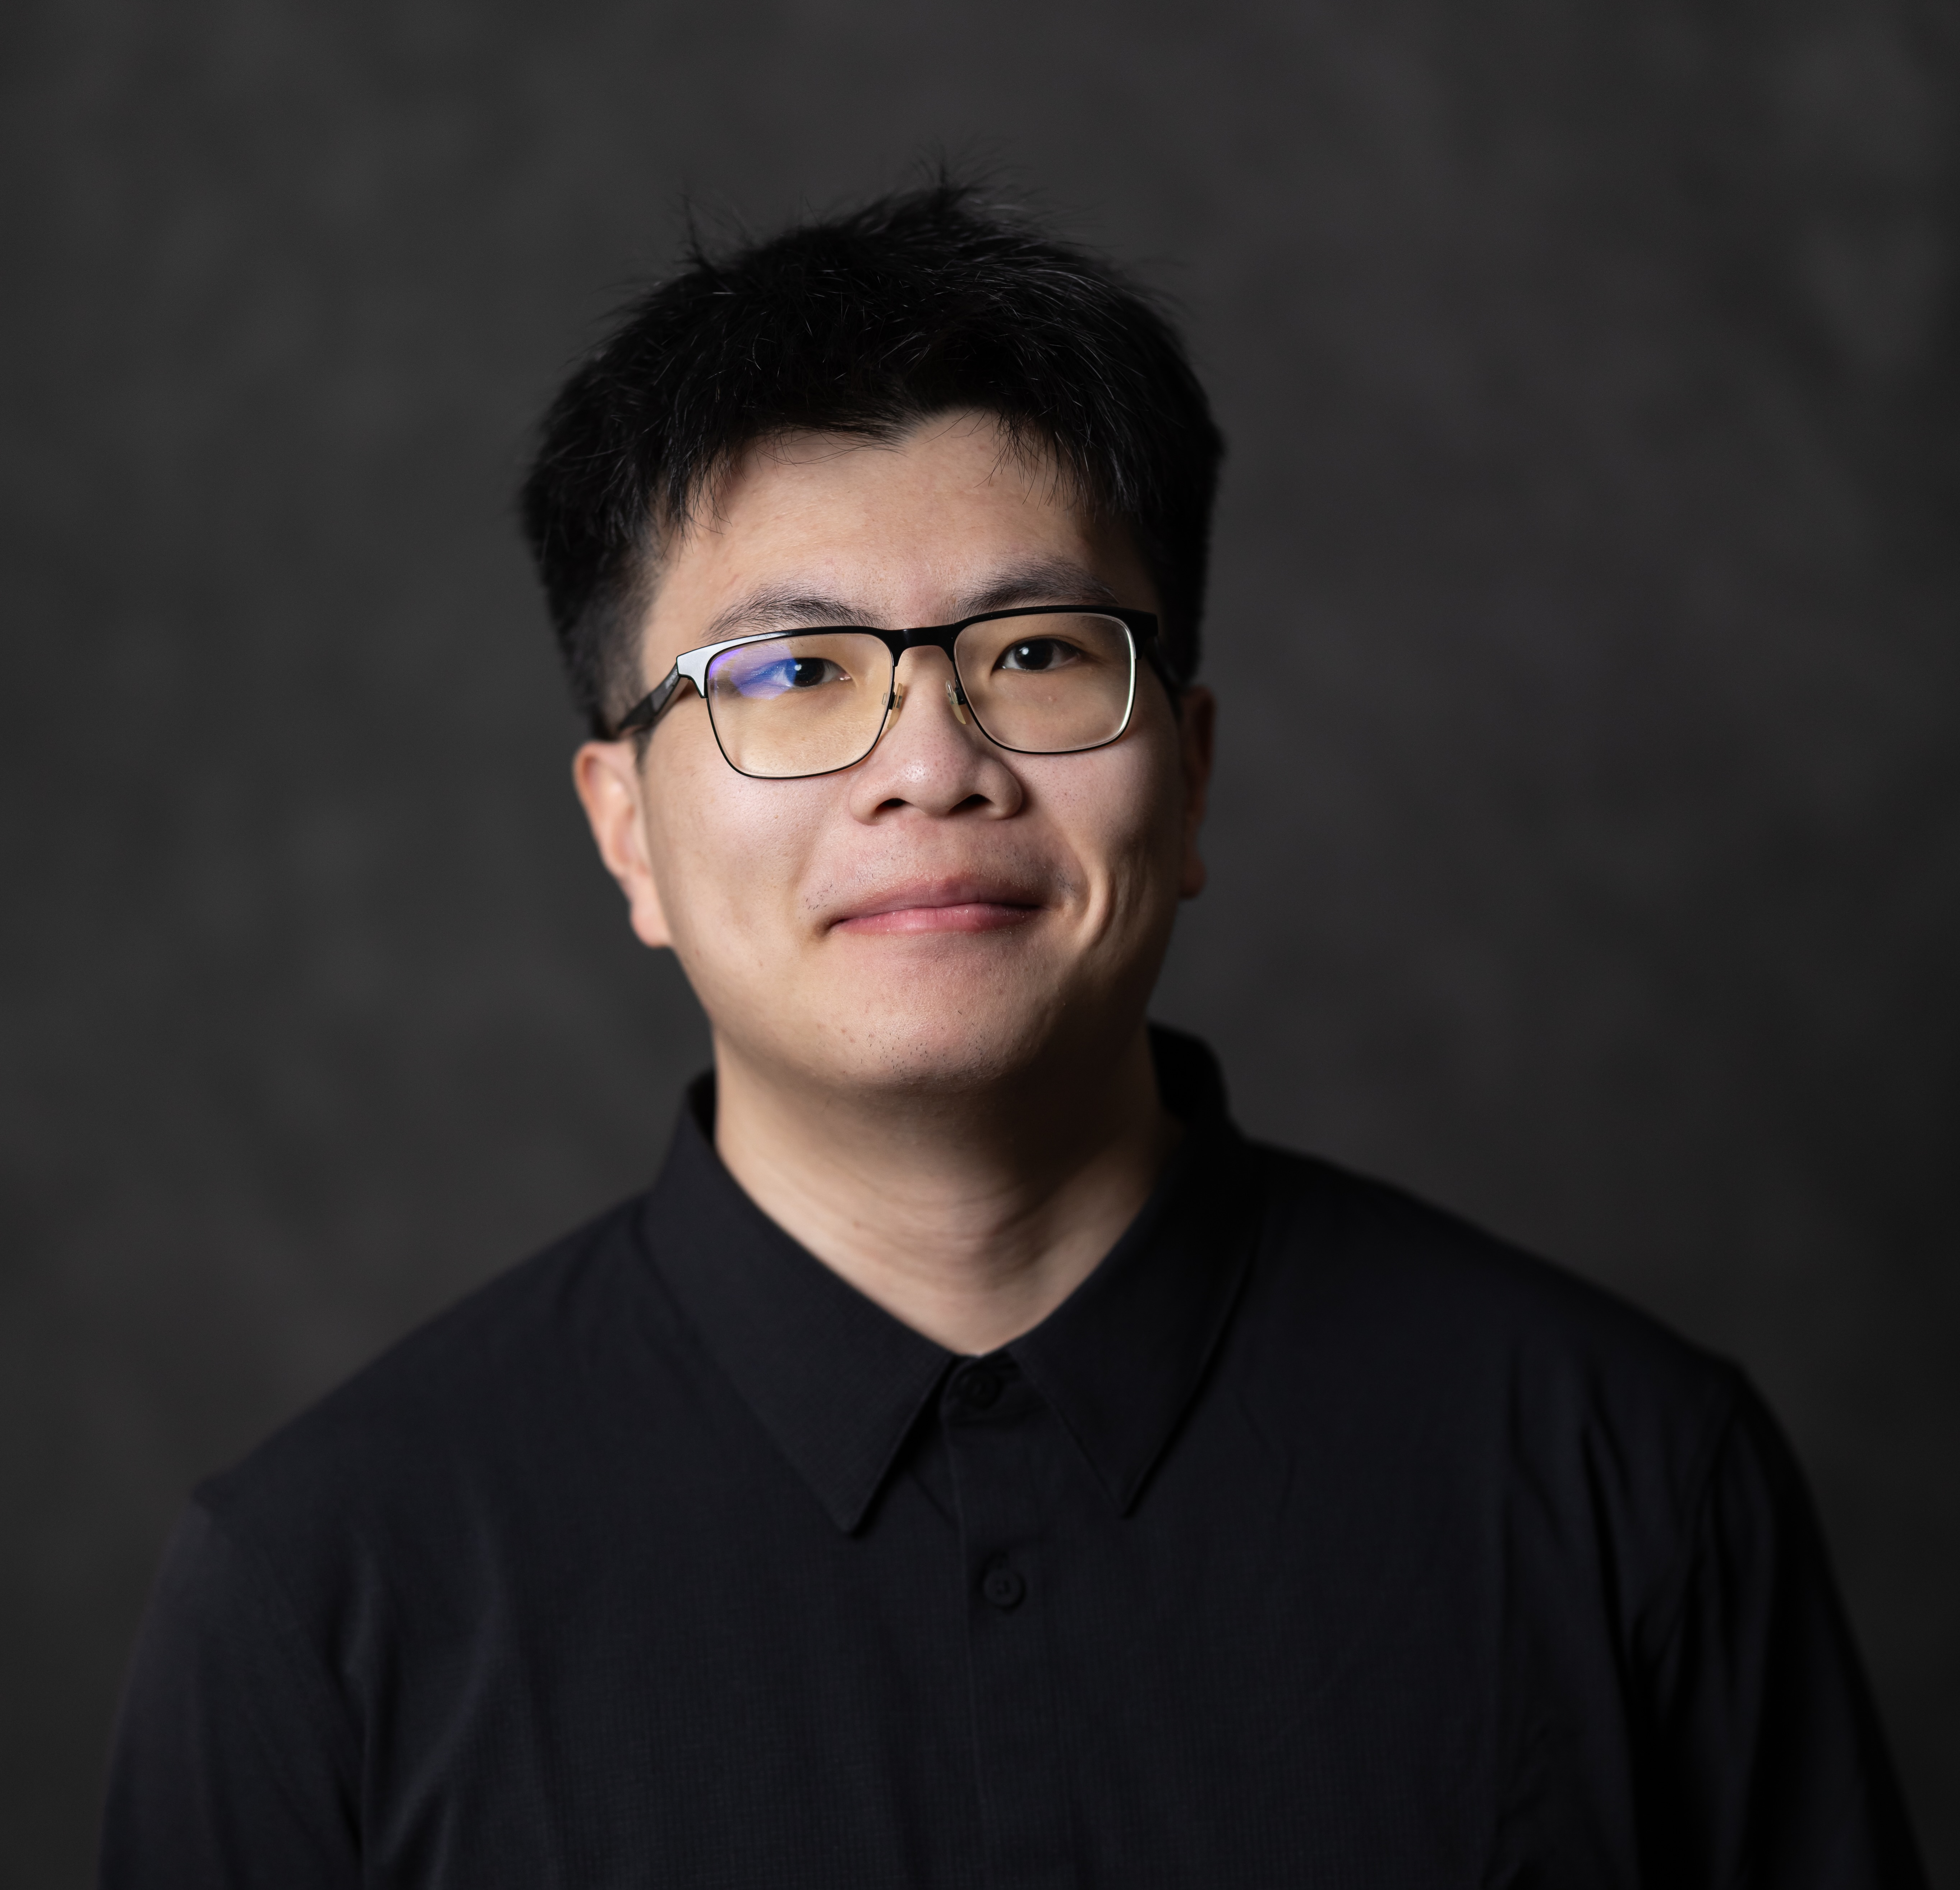
\includegraphics[width=3cm]{headshot_1.jpg}
\end{textblock*}
\vspace{-5pt}

{\zihao{4} {\textbf{相关经历}}}\vspace*{-6pt}\\
\rule{\textwidth}{0.4pt}
{\labelfont {\textbf{深圳高灯计算机科技有限公司, 深圳, 广东}}  \hspace{9.3cm} 2024 6月 - 8月}\\
\vspace{-11pt}\\
{\labelfont \textit{前端开发实习}  }\\
\vspace{-27pt}\\
{
\small
\begin{itemize}
\setlength\itemsep{1pt}
    \item 通过\textbf{Vue.js}界面和\textbf{集成第三方API}至内部数据库,提高利润跟踪效率,优化通行费与利润数据的访问流程。
    \item 与后端团队协作,优化现有赊销功能的逻辑和UI,并对接\textbf{微风企API},以更好满足企业风险评估信息收集的业务需求。
    % \item Developed a notification feature for the company's \textbf{WeChat Mini Program} (a widely used lightweight software platform in China) on the enterprise management side, providing alerts for transaction activities, fuel station price changes, and other updates, \textbf{enhancing} transaction tracking and \textbf{client engagement}.
    \item 开发\textbf{微信小程序(驿能加油车管端)}的通知页面,实现定价和交易提醒,提高交易跟踪效率。
    \item 优化内外部界面的UI和组件逻辑,开发并实现\textbf{Vue.js}界面以管理合作加油站的标识和名称。
    \item 与产品经理和UI设计师协调,深入分析需求.
\end{itemize}
}
{\labelfont \textbf{明尼苏达大学计算机网络研究组, 明尼阿波利斯, 明尼苏达州,美国}  \hspace{1.5mm}\hspace{4.1cm} 2023 5月 - 2024 5月}\\
\vspace{-11pt}\\
{\labelfont \textit{研究助理} }\\
\vspace{-27pt}\\
{
\small
\begin{itemize}
\setlength\itemsep{1pt}
    \item 使用\textbf{Python}分析1,711个Traceroute文件,揭示德国、意大利、西班牙和法国的数据漫游模式,并识别出法国Orange运营商的独特漫游模式.
    \item 利用\textbf{latex, panda}构建深入且富有洞察力的图表,可视化漫游模式和Traceroute数据摘要,增强研究分析,并支持\href{https://ieeexplore.ieee.org/document/10621234}{论文}的数据呈现,以第五作者身份发表该论文。
\end{itemize}
}


{\zihao{4} {\textbf{教育}}}\vspace*{-6pt}\\
\rule{\textwidth}{0.4pt}
{\labelfont \textbf{计算机科学硕士} \hspace{12.7cm} 2024 9月 - 2026 5月}\\
{\small 明尼苏达大学双城分校,明尼阿波利斯,明尼苏达州,美国
\hspace{5.5cm}
}
\vspace*{3pt}

{\labelfont \textbf{计算机科学学士} \hspace{12.7cm} 2022 1月 - 2024 5月}\\
{\small 明尼苏达大学双城分校,明尼阿波利斯,明尼苏达州,美国 \hspace{5.5cm}
\vspace{1.5pt}\\
\small 2023年秋季学期院长名单,托福TOEFL 103 \hspace{5.5cm}
}

\vspace*{5pt}
{\zihao{4} {\textbf{项目}}}\vspace*{-6pt}\\
\rule{\textwidth}{0.4pt}
{\labelfont \textbf{预算追踪助手},\textit{\href{https://github.com/csci5117s24/project-2-html-heroes-2}{GitHub链接}},(因该应用部署在微软Azure平台上,需要VPN进行访问)\hspace*{2.8cm}\hspace{2.4mm}\hspace{1.5mm}2024 5月}
{
\small
\vspace{-15pt}\\
\begin{itemize}
\setlength\itemsep{1pt}
    \item 与4人团队合作开发基于前端\textbf{React}和后端\textbf{Azure MongoDB}的Web应用,支持用户查看和管理支出和预算。
    \item 集成\textbf{微软Azure AI Form Recognizer}以从结账收据照片中提取总金额,简化用户输入支出的流程。
    \item 使用\textbf{ArmChart JS}库和\textbf{Tailwind CSS}设计美观的图表和界面,并结合\textbf{响应式网页设计},确保Web应用在不同屏幕尺寸的设备上良好呈现。
    \item 使用\textbf{Auth0}实现使用GitHub账号登录功能。该应用可通过\textit{\href{https://nice-ocean-02cf72b0f.5.azurestaticapps.net}{此链接}}访问并使用。
\end{itemize}
}

{\labelfont \textbf{活动雷达}, \textit{\href{https://github.com/csci5117s24/project-1-html-heroes}{GitHub链接}} \hspace*{13.3cm}\hspace{1mm}\hspace{1.5mm}2024 5月}
{
\small
\vspace{-15pt}\\
\begin{itemize}
\setlength\itemsep{1pt}
    \item 开发了一款Web应用,支持活动组织者创建和管理活动,同时允许用户浏览并订阅感兴趣的活动。使用\textbf{Flask}实现前后端集成,并采用\textbf{PostgreSQL}进行数据库管理。
    \item 集成\textbf{Google API},支持将活动添加至Google日历,并通过Google地图搜索活动地点。
\end{itemize}
}

{\labelfont \textbf{待办事项管理应用} \hspace*{13.82cm} \hspace{1.5mm}\hspace{1.5mm}2022 12月}
{
\small
\vspace{-27pt}\\
\begin{itemize}
\setlength\itemsep{1pt}
    \item 使用\textbf{HTML}、\textbf{CSS}和\textbf{JavaScript}实现前端,支持待办事项的管理和筛选。
    \item 使用\textbf{Node.js}、\textbf{MySQL数据库}和\textbf{Pug模板引擎}构建后端,负责数据处理和服务器端逻辑。
\end{itemize}
}

%\vspace*{1pt}
%{\labelfont \textbf{Related Coursework}}
%\\Machine Architecture and Organization\hspace{0.5cm}Advanced Programming Principles\hspace{0.5cm}Program %Design and Development\hspace{0.5cm}\\Algorithms and Data Structures\hspace{0.5cm}Internet %Programming\hspace{0.5cm}Introduction to Computer Networks\hspace{0.5cm}\\Dev Ops I: Network %Programming\hspace{0.5cm}Advanced Algorithms and Data Structures\hspace{0.5cm}Discrete Structures of Computer %Science


% \vspace*{1pt}
{\zihao{4}{\textbf{相关技能}}}\vspace*{-6pt}\\
\rule{\textwidth}{0.4pt}
{
{\labelfont \textbf{前端框架工具 \& 数据库}}: React, Node.js, Flask, Vue.js, PostgreSQL, Azure MongoDB, Webpack, Jest, GraphQL
\vspace*{1.5pt}\\
{\labelfont \textbf{编程语言}}: Typescript, JavaScript, HTML, CSS, C, C++, Python, Java, Ocaml
\vspace*{1.5pt}\\
{\labelfont \textbf{其他}}: Tailwind CSS, RESTful APIs, Git, Docker, Vscode, Apache Tomcat, Google API, Linux, Agile
}

\vspace*{3pt}
{\zihao{4} {\textbf{论文发表}}}\vspace*{-6pt}\\
\rule{\textwidth}{0.4pt}
Rostand A. K. Fezeu, Claudion Fiandrino, Eman Ramadan, Jason Carpenter,\textit{\textbf{ Daqing Chen}}, Yiling Tan, Joerg Widmer, Feng Qian, and Zhi-Li Zhang, ``Roaming across the European Union in the 5G era: Performance, challenges and opportunities,'' in \textit{Proceedings of the IEEE International Conference on Computer Communications (INFOCOM '24)}, Association for Computing Machinery




% {\labelfont \textbf{Drone Simulation System} \hspace*{12.5cm}\hspace{1.5mm}\hspace{1.5mm}Dec 2022}
% {
% \small
% \begin{itemize}
% \setlength\itemsep{-2.5pt}
%     \item Collaborated with team of three and worked in a sprint to develop a drone simulation system using C++.
%     \item Implemented Decorator design pattern to wrap up the drone with a battery, enabling the behaviors related to battery life.
%     \item  Followed development processes including version control, code reviews, project management, documentation, and software testing.
% \end{itemize}
% }
% {\labelfont \textbf{HTTP Web Server} \hspace*{7.8cm}\textbf{Dev Ops I: Network Programming} \hspace{1.5mm}\vline\hspace{1.5mm}May 2023}
% {
% \small
% \begin{itemize}
% \setlength\itemsep{-2.5pt}
%     \item Built this web server using standard C socket library, concurrency and CGI.
%     \item Parsed users' request from browser and rendered the page with graphics back inside the server.
% \end{itemize}
% }


% {\labelfont \textbf{Semantic Segmentation for Object Identification} \hspace*{8.75cm} Dec 2019}
% {
% \small
% \begin{itemize}
% \setlength\itemsep{-2.5pt}
%     \item Designed a pipeline from scratch in C++ to perform instance segmentation on simple, unknown images.
%     \item Used traditional CV techniques using OpenCV to partition and categorize objects without any priors.
% \end{itemize}
% }

% \noindent\rule{\textwidth}{1pt}\vspace*{5pt}

\end{document}
